\documentclass[11pt]{article}

\usepackage[letterpaper,margin=0.78in]{geometry}
\usepackage[T1]{fontenc}
\usepackage[utf8]{inputenc}
\usepackage{lmodern}
\usepackage{microtype}
\usepackage{parskip}
\usepackage{amsmath,amssymb}
\usepackage{array,booktabs,longtable,tabularx}
\usepackage{enumitem}
\usepackage{xcolor}
\usepackage{graphicx}
\usepackage{tikz}
\usetikzlibrary{arrows.meta,calc,positioning,shapes.geometric}
\usepackage{fancyhdr}
\usepackage{hyperref}

\definecolor{duneblue}{HTML}{004C97}
\definecolor{dunelightblue}{HTML}{DCEAF7}
\definecolor{dunegreen}{HTML}{2E7D32}
\definecolor{dunelightgreen}{HTML}{E8F3E8}
\definecolor{duneorange}{HTML}{E87722}
\definecolor{dunelightorange}{HTML}{FFF0E5}
\definecolor{dunered}{HTML}{B3261E}
\definecolor{dunelightred}{HTML}{FCE8E6}
\definecolor{dunegray}{HTML}{4F5B66}
\definecolor{dunelightgray}{HTML}{F1F3F4}

\hypersetup{
  colorlinks=true,
  linkcolor=duneblue,
  urlcolor=duneblue,
  citecolor=duneblue,
  pdftitle={GIZMO Ground-Reference Monitoring Operations Guide -- Full Guide},
  pdfauthor={Manuel Arroyave}
}

\pagestyle{fancy}
\fancyhf{}
\lhead{DUNE Far Detector --- GIZMO operations guide}
\rhead{Integration and commissioning draft}
\cfoot{\thepage}
\setlength{\headheight}{14pt}
\setlength{\emergencystretch}{3em}

\setlist[itemize]{leftmargin=1.45em,itemsep=2pt,topsep=3pt}
\setlist[enumerate]{leftmargin=1.65em,itemsep=4pt,topsep=3pt}
\setlist[description]{leftmargin=1.2em,labelindent=0em,itemsep=3pt}

\newcommand{\GIZMO}{\textsc{GIZMO}}
\newcommand{\DetectorGround}{\textit{Detector Ground}}
\newcommand{\InfrastructureGround}{\textit{Cavern/Building Ground}}
\newcommand{\checkbox}{\raisebox{0.15ex}{\fbox{\rule{0pt}{1.15ex}\rule{1.15ex}{0pt}}}}
\newcommand{\TBD}{\textcolor{dunered}{\textbf{TBD}}}

\newcommand{\callout}[3]{%
  \begin{center}
  \fcolorbox{#1}{#2}{%
    \begin{minipage}{0.92\linewidth}
      #3
    \end{minipage}}
  \end{center}
}
\newcommand{\danger}[1]{\callout{dunered}{dunelightred}{\textbf{STOP / SAFETY:} #1}}
\newcommand{\warning}[1]{\callout{duneorange}{dunelightorange}{\textbf{Important:} #1}}
\newcommand{\operatornote}[1]{\callout{duneblue}{dunelightblue}{\textbf{Operator note:} #1}}
\newcommand{\good}[1]{\callout{dunegreen}{dunelightgreen}{\textbf{Expected result:} #1}}

\newcolumntype{Y}{>{\raggedright\arraybackslash}X}
\newcolumntype{L}[1]{>{\raggedright\arraybackslash}p{#1}}

\title{%
  \vspace{-1.2cm}
  \textcolor{duneblue}{\Huge\bfseries GIZMO Ground-Reference Monitoring Operations Guide}\\[3mm]
  \Large Connection, commissioning, and monitoring during construction and operation\\[1mm]
  \large DUNE Far Detector
}
\author{Manuel Arroyave\\[1mm]\small Full guide: installation, contractor coordination, and operation}
\date{Public review update of October 5, 2026}

\begin{document}
\maketitle

This guide explains how the deployed Kria GIZMO is connected, checked, and used during construction. It is for the contractor work lead, FNAL I\&I/GIZMO, the electrical lead, and the Slow Controls/Detector Protection System (SC/DPS) team.

Use it with the current SOP004, grounding drawings, rack Operational Readiness Clearance (ORC), and work plan. Those documents set the electrical work controls, including lockout/tagout (LOTO). This is a public review draft; the site settings and responsibilities in Section~\ref{sec:site-record} still need to be completed.

\danger{Keep the required safety-ground path intact. Only authorized electrical personnel may change grounding connections. Never lift a safety ground to clear a GIZMO alarm.}

\tableofcontents
\clearpage

\section{Grounding and measurement: the terms used here}

\begin{description}
  \item[Detector Ground] The cryostat steel vessel and the metal structures bonded to it. It is the electrical reference for detector electronics.
  \item[Building Ground] The bonded cavern and building infrastructure, including the protective grounding used by conventional electrical equipment.
  \item[Bond] A deliberate electrical connection between metal parts. The \emph{construction bond} is the Building Ground connection required while the contractor works on the cryostat and beam structure.
  \item[Safety-ground path] The connection designed to carry fault current so electrical protection can operate. The detector arrangement includes an approved saturable-inductor assembly. Its inductance limits small AC noise currents; under a large fault current, saturation reduces its impedance. The released drawing defines the complete protective path.
  \item[Isolation] The absence of unwanted connections between Detector Ground and Building Ground, while the approved safety-ground path remains intact.
  \item[Impedance] Opposition to AC current at a stated frequency. GIZMO uses an AC measurement to detect changes in resistive connections and capacitive coupling between the grounds.
  \item[Baseline] The accepted measurement for a known grounding arrangement, frequency, and calibration. Compare results only when those conditions match.
  \item[Handback] The point at which testing is finished, the required work grounding is restored and verified, and the contractor lead is told that the area is released for work.
\end{description}

\subsection{Why the metal structure must stay grounded}

Friction during material handling, moving belts, or dust flow can generate static charge. An isolated metal structure can retain that charge until it discharges through a person or electronics. Grounding drains the charge and reduces the risk of electrostatic discharge (ESD).

There is also a separate electrical hazard: a damaged powered tool or cable can energize the structure. The safety-ground path must carry the resulting fault current so protective devices can operate. A connection that drains static charge is not, by that fact alone, adequate fault protection.

Keep the required Building Ground bond connected during contractor work. Corrosion, loose clamps, and damaged conductors can weaken that connection, so inspect and verify it at shift start and handover.

\subsection{Why GIZMO tests must be repeated}

Construction changes the electrical arrangement. Cables, scaffolding, temporary leads, piping, and new metalwork can introduce unwanted connections or change capacitance. These changes can affect detector noise performance and become harder to find after later work covers the area.

Repeat the GIZMO tests at agreed intervals and after work that could change the arrangement. A safety-bond check verifies the required protective connection. A GIZMO isolation test looks for unwanted paths and changes in coupling. One does not replace the other.

\section{How the measurement works}\label{sec:measurement}

GIZMO injects a small AC signal between the two grounds. A Pearson current transformer (CT) measures the portion returning through the intended safety-ground conductor. Another conductive path can divert current around that route and change the reported impedance.

The reading does not locate the connection. Its meaning depends on the actual grounding arrangement. The figure shows the measurement principle; use the released drawing for installation and switching.

\begin{figure}[htbp]
\centering
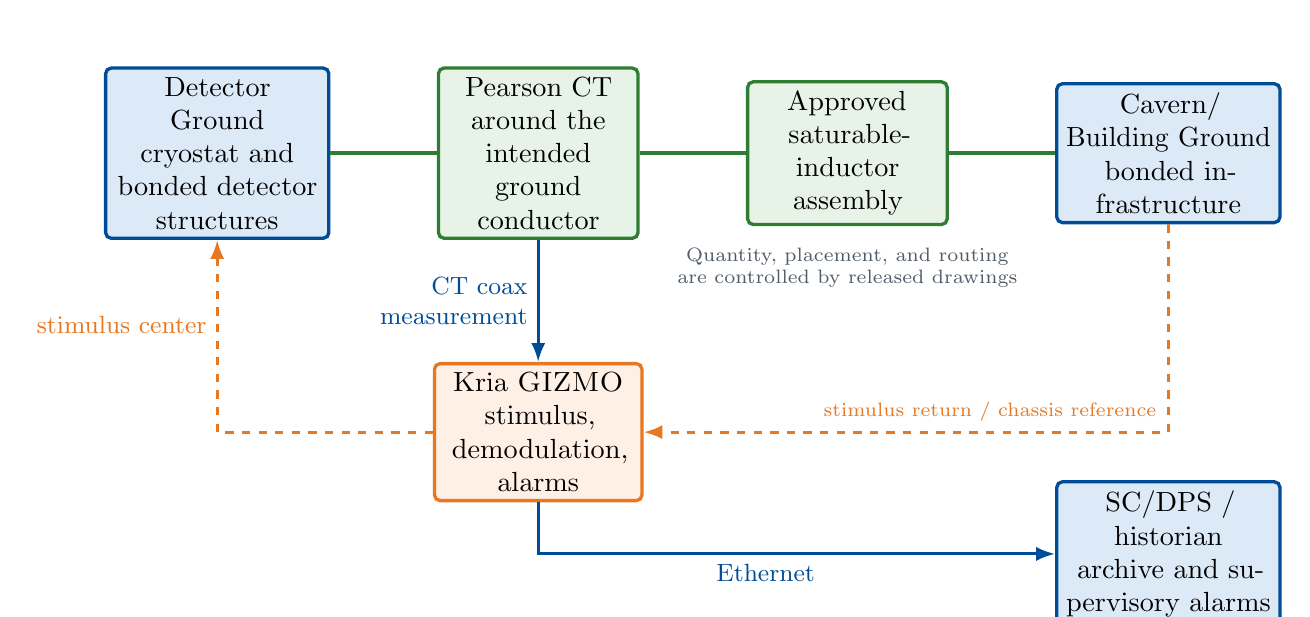
\begin{tikzpicture}[
  >=Latex,
  node distance=1.2cm and 1.35cm,
  box/.style={draw=duneblue,very thick,rounded corners=2pt,fill=dunelightblue,
              align=center,minimum height=1.25cm,text width=2.6cm},
  safety/.style={draw=dunegreen,very thick,rounded corners=2pt,fill=dunelightgreen,
                 align=center,minimum height=1.25cm,text width=2.3cm},
  monitor/.style={draw=duneorange,very thick,rounded corners=2pt,fill=dunelightorange,
                  align=center,minimum height=1.25cm,text width=2.4cm},
  wire/.style={line width=1.5pt,dunegreen},
  signal/.style={line width=1.1pt,duneblue,-{Latex[length=2.4mm]}},
  stimulus/.style={line width=1.1pt,duneorange,dashed,-{Latex[length=2.4mm]}}
]
  \node[box] (det) {Detector Ground\\cryostat and bonded detector structures};
  \node[safety,right=of det] (ct) {Pearson CT\\around the intended ground conductor};
  \node[safety,right=of ct] (si) {Approved saturable-\\inductor assembly};
  \node[box,right=of si] (bldg) {Cavern/\\Building Ground\\bonded infrastructure};
  \node[monitor,below=1.55cm of ct] (gizmo) {Kria \GIZMO{}\\stimulus, demodulation, alarms};
  \node[box,below=3.25cm of bldg] (sc) {SC/DPS / historian\\archive and supervisory alarms};

  \draw[wire] (det) -- (ct) -- (si) -- (bldg);
  \draw[signal] (ct) -- node[left,align=right,font=\small]{CT coax\\measurement} (gizmo);
  \draw[stimulus] (gizmo.west) -| node[pos=0.78,left,font=\small]{stimulus center} (det.south);
  \draw[stimulus] (bldg.south) |- node[pos=0.67,above,font=\scriptsize]{stimulus return / chassis reference} (gizmo.east);
  \draw[signal] (gizmo.south) |- node[pos=0.72,below,font=\small]{Ethernet} (sc.west);

  \node[below=0.15cm of si,font=\scriptsize,text=dunegray,align=center]
    {Quantity, placement, and routing\\are controlled by released drawings};
\end{tikzpicture}
\caption{Conceptual measurement topology. The CT must observe the intended return path; any parallel detector-to-infrastructure connection changes the measured signal.}
\label{fig:concept}
\end{figure}

The planned initial installation uses one saturable inductor. Verify its protection, CT routing, and connection between Detector Ground and Cavern/Building Ground against the released installation drawing. The required construction bond and any knife-switch arrangement are defined by that drawing; the conceptual figure does not authorize switching them.

\section{Who does what}

\begin{tabularx}{\linewidth}{@{}L{0.25\linewidth}Y@{}}
\toprule
Role & Responsibility \\
\midrule
Contractor work lead & Describes the planned work and recent changes, arranges shift bond checks, clears the agreed test area, and acknowledges handback. \\
Electrical lead & Controls grounding work and switching. Assigns authorized electrical personnel to verify the safety path, establish the test arrangement, and verify restoration. \\
FNAL I\&I/GIZMO & Takes and interprets GIZMO measurements, checks the instrument and dashboard, runs isolation tests, provides local fallback measurements, and records results. \\
Activity coordinator & Agrees work and test windows with the contractor and FNAL, tracks the work package, and coordinates release of the area. \\
SC/DPS team & Maintains the controls connection, display, timestamps, history, and alarms for missing or invalid data. \\
Facility support & Maintains the instrument and mine-network support needed for remote measurements and the approved local alternative. \\
\bottomrule
\end{tabularx}

Name the people filling these roles for each shift. The contractor's bond checker must be trained for the specified method. GIZMO readings, calibration, and settings remain with FNAL I\&I/GIZMO.

\section{Working with the contractor}
\label{sec:contractor}

\subsection{Agree the work and test windows}

Before the shift, the contractor lead, electrical lead, activity coordinator, and FNAL I\&I/GIZMO agree what work is planned, which bonds must be connected, and when FNAL can test. Set recurring windows before, after, or between shifts. Add a test after work that could change grounding or coupling, and before new work covers an area that may need inspection.

The work plan must state the test interval, settling time, limits, named contacts, and response to a failed or missed test. Record the next test time. These values depend on the installation and must be assigned by the responsible site leads.

\begin{tabularx}{\linewidth}{@{}L{0.24\linewidth}Y@{}}
\toprule
Arrangement & What the reading can tell you \\
\midrule
Contractor work & The required Building Ground bond is connected and verified. A low reading or active alarm may be expected, and that bond can hide a second unwanted connection. \\
FNAL isolation test & Authorized personnel set the approved switch/tagout arrangement while keeping the permanent safety path intact. FNAL compares the result with the baseline for this arrangement. \\
Welding or another planned bond & The added connection may change the reading. Record which bonds are present and use the welding procedure in Section~\ref{sec:welding}. \\
\bottomrule
\end{tabularx}

The knife switch must be identified by its function in the released drawing. This guide does not assume which contact may be opened. If the safe test arrangement is unclear, resolve it with the electrical lead before switching.

\subsection{At shift start and handover}

\begin{enumerate}
  \item The contractor lead arranges an inspection of the accessible grounding cables, clamps, and connections. Report damage, looseness, corrosion, or paint obstructing contact.
  \item The designated checker verifies the required Building Ground bond using the specified instrument, test points, method, and acceptance limit. Never use resistance mode on an energized circuit. A continuity beep alone is not a pass.
  \item Confirm the knife-switch position and tagout status against the work plan. Report any mismatch to the electrical lead.
  \item Tell FNAL what changed since the previous test: new metalwork, cables, temporary bonds, welding returns, or moved equipment. Confirm the next test window.
  \item Record the checker, time, bond result, grounding arrangement, and open issues in Procore Daily Log $>$ GIZMO.
\end{enumerate}

\subsection{During a FNAL test window}

\begin{enumerate}
  \item The contractor lead confirms that the agreed area is available and affected work is paused. Clear tools and cords that could bridge the grounds during the test.
  \item Authorized electrical personnel establish and record the switch/tagout arrangement. The permanent safety path, including the approved inductor assembly, stays effective throughout the test.
  \item FNAL waits the specified settling time, then checks data age, quality, calibration, frequency, and alarm status. Record resistance or HIGH Z, valid capacitance, and coupling diagnostics. Compare with the limits and the previous test under the same conditions.
  \item If the result is unexpected, FNAL and the electrical lead investigate with the contractor lead. Start with the work done since the last good test. Record the finding and retest after correction.
\end{enumerate}

\subsection{Before the contractor resumes work}

Restore the required Building Ground connection and have it verified by the electrical lead's designated person. Complete tagout closeout, record the FNAL test result, and obtain release from the person named in the work plan. The contractor lead acknowledges the restored arrangement and the next test time before work resumes.

A failed or missed isolation test needs a recorded decision from the responsible lead under the work plan; it cannot be entered as a pass. A safety-ground defect must be corrected and verified before affected work restarts. Use Section~\ref{sec:response} when the grounding or measurement is uncertain.

\section{Before installation or a connection change}

Use this check after installation or a change to the rack, grounding, CT, inductor, stimulus connection, or firmware.

\begin{enumerate}
  \item Check the current SOP004, work plan, grounding drawing, cable schedule, CT orientation, inductor/protection drawing, and rack ORC. Record the equipment and configuration identifiers in Section~\ref{sec:site-record}.
  \item Identify and label Detector Ground, Building Ground, the conductor through the CT, both sides of the inductor, and the stimulus and return points. Follow the drawing and text labels; wire color alone does not establish a connection's function.
  \item With the circuits in the safe state specified by the work plan, inspect enclosures, connectors, strain relief, and conductor clearances. Verify the rack and chassis bonds and the detector safety-ground path.
  \item Check that the CT surrounds the intended conductor and that any parallel construction or welding bond is documented. Check tools, temporary leads, shields, pipes, and jumpers against the declared arrangement.
  \item Check that the beacon is visible and the audible alarm is suitable for the work area.
\end{enumerate}

Do not energize or inject the test signal if a conductor is unidentified, a required bond is missing or unverified, the installation differs from the drawing, or the software/configuration cannot be identified. Resolve the discrepancy with the electrical lead and FNAL before proceeding.

Post a short reference on the rack door with the rack and ORC identifiers, labeled ground points, expected alarm indications, current contacts, and a link to the work procedure and Procore log. Include the safety-ground instruction from the first page.

\section{Connection sequence}

Make these connections with the equipment de-energized. The current installation has no power distribution unit (PDU). Use the installed GIZMO power supply and verify its connections against the site electrical procedure. Authorized electrical personnel handle fixed grounding conductors and protection devices.

\begin{enumerate}
  \item \textbf{Safety-ground assembly.} The authorized electrical worker installs or verifies the approved Detector Ground--CT--saturable-inductor/protection--Cavern/Building Ground path. Do not open this path as part of routine \GIZMO{} work.

  \item \textbf{CT signal.} Connect the approved coaxial cable from the Pearson CT output to the \GIZMO{} connector designated \textsc{CT INPUT}. Verify both endpoint labels and cable ID.

  \item \textbf{Stimulus.} Connect the stimulus output using the approved custom cable:
  \begin{itemize}
    \item the center conductor goes to the designated Detector Ground-side injection point;
    \item the outer conductor/return is bonded to the designated rack or Cavern/Building Ground point.
  \end{itemize}
  Do not improvise this cable or move the injection point without repeating characterization.

  \item \textbf{Alarm outputs.} Connect the warning beacon and audible alarm to the labeled \GIZMO{} outputs. Do not use an alarm-power connector as a general auxiliary supply.

  \item \textbf{Network.} Connect the Kria \GIZMO{} Ethernet port to the assigned detector controls network switch port.

  \item \textbf{DC power.} Connect the approved NRTL-listed AC/DC converter to the Kria chassis. Verify supply voltage and current rating against the installed chassis label before connection.

  \item \textbf{AC input.} Connect the GIZMO power supply to the assigned AC supply point using the approved cable. Verify the required protective-earth connections before energizing.
\end{enumerate}

Work that changes or temporarily bypasses the safety-ground conductor needs a separate electrical procedure. The sequence above does not cover that operation.

\subsection{Independent connection verification}

Before power-up, have a second qualified person check each connection against the drawing and record initials:

\begin{center}
\begin{tabularx}{0.94\linewidth}{@{}Y L{0.19\linewidth} L{0.19\linewidth}@{}}
\toprule
Connection & Installed by & Verified by \\
\midrule
CT output $\rightarrow$ \GIZMO{} CT input & & \\
Stimulus center $\rightarrow$ approved Detector Ground-side point & & \\
Stimulus return/chassis $\rightarrow$ approved Cavern/Building Ground & & \\
Beacon and audible alarm outputs & & \\
Kria network connection & & \\
GIZMO DC supply rating, cable, and AC supply point & & \\
Safety path and CT routing match released drawing & & \\
\bottomrule
\end{tabularx}
\end{center}

\section{Power-up}

Before applying power, confirm that the connection check is signed, the actual grounding arrangement is recorded, and the software, configuration, and calibration match the site record. Have storage and the required remote copies of the data ready. Keep the stimulus disabled until the electrical lead authorizes it.

\begin{enumerate}
  \item Energize the installed GIZMO power supply as specified in the site procedure. Check the normal power indications. Stop and de-energize safely if there is abnormal heat, sound, odor, or smoke.
  \item Wait the specified boot time. Check that \texttt{gizmo.target} and its required services are healthy, and record the runtime and model versions.
  \item From the controls host, connect to the assigned OPC~UA endpoint and verify the device identity and certificate. Check that source timestamps advance, the clock is correct, and data age is within the site limit.
  \item Confirm the waveform, frequency, amplitude limit, and calibration. Use the site startup procedure to start acquisition and enable the stimulus when the electrical lead authorizes it.
  \item Check that measurements and alarm status have Good quality, sequences advance, and the historian is writing data. Check that required remote copies are receiving updates.
  \item Compare the reading and alarm with the baseline for the actual grounding arrangement. A reading taken with the construction bond connected must be compared with that state, not with the isolation-test baseline.
\end{enumerate}

The instrument is ready when these checks pass. Release of the contractor's work area is a separate step, described in Section~\ref{sec:contractor}. The site record must supply the exact startup, stimulus-control, and recovery commands; the public software interface alone does not define the field sequence.

\section{Commissioning and baseline}

Commissioning establishes the response of the installed cryostat, safety path, CT, stimulus cable, and instrument. Keep the resulting baseline with its grounding arrangement, frequency, and calibration so later readings can be compared with it.

\subsection{Measurements to make}

Use the test fixture and electrical controls specified in the commissioning plan. Measure:

\begin{itemize}
  \item the reference response and its normal variation;
  \item known resistances spanning the isolation and alarm conditions;
  \item known capacitances representative of the installation;
  \item response over the permitted frequency range;
  \item response with representative construction equipment on and off;
  \item operation of the beacon, audible alarm, controls alarm, and event logging.
\end{itemize}

A reference or ``open'' measurement is a test-fixture condition; it does not instruct anyone to disconnect the permanent safety ground.

\subsection{Frequency and threshold}

Choose a frequency that avoids installation resonances and strong equipment-noise lines, separates the reference response from known shorts, and gives stable measurements within the permitted stimulus and touch-voltage limits. Record the scan, chosen frequency, waveform, amplitude, uncertainty, calibration identifier, and approver.

The recorded operating frequency is 1436 Hz. Confirm it against the installed configuration and calibration. A different frequency, stimulus amplitude, CT, cable route, inductor, or major bonding change needs review and may require a new baseline.

Set the alarm threshold from these measurements. Document the separation from normal variation and the margin for the highest-resistance unwanted connection that must be detected. A threshold change is an engineering decision; it is not a way to clear an unexplained alarm.

\section{Routine monitoring}

FNAL I\&I/GIZMO checks the instrument at shift start and handover. Exchange the results with the contractor lead and review the contractor checks in Section~\ref{sec:contractor}.

\begin{enumerate}
  \item Confirm that the work record matches the bonds and activities actually present, and that the next test window is agreed.
  \item Check source time, data age, quality, alarm, and range. Interpret the result using Section~\ref{sec:response}.
  \item Compare the frequency, calibration, threshold, and configuration with the shift reference.
  \item Review the previous 12 hours for changes, drift, gaps, or work windows that were not closed.
  \item Check the historian, storage space, remote copies, and archive status. Record the result and any action needed in Procore Daily Log $>$ GIZMO.
\end{enumerate}

\subsection{What the operator needs on the display}

Show the reading or HIGH Z, alarm and reason, source time, data age, quality, and recent trend together. Make the frequency, threshold, calibration/configuration identifiers, and instrument/network status accessible. FNAL should also be able to inspect the in-phase and quadrature (I/Q) signals used to calculate the result.

Show the actual work and bond arrangement alongside the measurements, with the person or system that supplied it and the time it was recorded. GIZMO does not know which contractor is working or whether a bond was authorized. Appendix~\ref{sec:controls-reference} lists the instrument fields and the information supplied by other systems.

\subsection{What to record}

Use Procore for the human record: shift checks, changes in work or bonding, test times and results, problems, corrective action, and handback. Link the before/after plots and data archive. Keep raw measurements in the historian; the storage and backup details are in Appendix~\ref{sec:controls-reference}.

\section{Welding and other planned bonds}
\label{sec:welding}

A welding return or temporary bond may intentionally connect the grounds. That connection can produce a low reading or an alarm and hide another unwanted path. Record when the connection is made, which work requires it, and when it is removed or left in its required final state.

\subsection{Before work}

\begin{enumerate}
  \item The contractor lead and activity coordinator confirm the work package, location, responsible crew, grounding arrangement, and start/end window. The electrical lead verifies the welding return and temporary bonds against the plan.
  \item FNAL records the pre-work reading and alarm after the required settling interval. If the construction bond must remain connected, record that condition and arrange a separate window for any required isolation test.
  \item Confirm that measurements and history will continue during the work. If annunciation must be inhibited, use the site's alarm-management procedure. Record who authorized it and its duration; preserve the raw alarm, quality, and timestamps.
\end{enumerate}

GIZMO does not verify welding-current routing. Do not disconnect the CT, stimulus, or monitor to silence an expected alarm.

\subsection{During work}

Record the actual time the bond becomes effective. Check for the response expected from that arrangement; an existing construction bond may hide the effect of the new connection. If a predicted change is absent, pause that step and have FNAL and the electrical lead check the measurement path.

Continue checking data freshness, instrument health, and logging. Record additional bonds, cable changes, moves, and pauses. Apply Section~\ref{sec:coverage-response} if valid measurements are lost.

\subsection{After work}

\begin{enumerate}
  \item The contractor lead confirms the activity has stopped. Authorized personnel remove temporary welding leads or put them in their specified final state. Retain the required construction bond and permanent safety path.
  \item FNAL checks the response against the required post-work arrangement for the specified settling and recovery intervals. If the construction bond remains, isolation must be checked in a separate authorized test window.
  \item If the reading does not recover as expected, inspect the recent work with the electrical lead and FNAL. Check temporary leads, cable shields, piping, scaffolding, and other new connections.
  \item Record the result, any pending test and the responsible lead's decision, and the before/after plot. Close the work window after the electrical lead and activity coordinator accept the arrangement and the contractor lead acknowledges handback.
\end{enumerate}

\section{What the conditions mean and what to do}
\label{sec:response}

Read the measurement with its source time, quality, and actual bond arrangement. \texttt{Good} means the instrument reports valid data; it does not certify personnel safety. \texttt{Alarm.Active} is the device's alarm decision, based on its resistance and phase logic. The beacon follows that decision and does not diagnose an open safety ground.

\begin{longtable}{@{}L{0.27\linewidth}L{0.66\linewidth}@{}}
\toprule
Condition & Meaning and action \\
\midrule
\endhead
Safety bond missing, damaged, or unverified & Stop affected work, keep clear, and notify the electrical and contractor leads. Correct the defect and verify the bond before authorized handback. Neither a GIZMO reading nor a dark beacon establishes that this connection is sound. \\
\addlinespace
Low reading or active alarm with a documented construction/welding bond & This may be the expected response to that bond. Confirm the work package, connections, and time window with the contractor lead. Continue monitoring and the scheduled isolation tests; another unwanted path may be hidden. \\
\addlinespace
Unexpected alarm during an isolation test or isolated operation & A new path or another configured alarm condition may be present. Pause further work that could change the connections. Record the time and alarm reason; ask FNAL and the electrical lead to investigate with the contractor work lead. \\
\addlinespace
Good-quality HIGH Z & This is a valid range indication, not an exact resistance. Record HIGH Z without substituting a number. Accept it only where it meets the test criteria for that arrangement; it does not prove the safety bond is intact. \\
\addlinespace
Reading changes but no alarm appears & A connection or capacitive coupling may have changed without triggering the alarm. Record the time and simultaneous work. FNAL compares the signals and baseline before deciding whether correction or a new characterization is needed. \\
\addlinespace
Stale timestamp, missing samples, or Uncertain/Bad quality & There is no reliable current result. Retain the last sample with its timestamp and status, record the gap, and use the coverage response below. Do not mark a required check passed. \\
\addlinespace
Invalid range, clipping, implausible readings, or frequency mismatch & The measurement setup or instrument may be wrong. FNAL checks the CT, stimulus, configuration, and calibration. Do not interpret an invalid result as good isolation. \\
\addlinespace
No alarm during a test that should trigger it & The alarm chain has not passed its check. FNAL verifies the fixture, settings, CT/stimulus connections, beacon, audible output, and controls reporting before releasing the instrument for routine use. \\
\bottomrule
\end{longtable}

\subsection{When remote measurements are unavailable}
\label{sec:coverage-response}

Facility support must maintain remote service and an approved local alternative so monitoring outages do not unnecessarily delay the contractor. FNAL performs and records the local measurements; the contractor is not responsible for instrument or network recovery.

The response depends on the work in progress:

\begin{itemize}
  \item If no activity depends on the missing measurements, record the outage and begin recovery. Unrelated work does not stop solely because the remote report is stale.
  \item If the activity needs monitoring, use the approved alternative only if it provides the coverage required by the work plan. Otherwise pause that activity until coverage is restored.
  \item If a scheduled test or handback check is missed, tell the contractor lead, electrical lead, and activity coordinator. Arrange a local test. If that is unavailable, the responsible lead must decide under the work plan whether the affected work can proceed, and record that decision.
\end{itemize}

Log the last valid sample, missed window, fallback method and results, recovery owner, and next test time. Escalate persistent or repeated outages to facility support and SC/DPS. An unsafe or unverified safety bond always follows the first row of the table above, regardless of monitoring availability.

\subsection{Finding an unwanted connection}

Start with what changed before the reading changed. The contractor lead identifies the work and arranges access; FNAL takes the measurements; the electrical lead controls any grounding changes. Disconnect candidate paths only through the responsible system owner and the electrical work procedure. Record the cause, correction, repeat-test result, and handback together.

\section{Shutdown and maintenance}

\begin{enumerate}
  \item Agree the outage with the contractor lead and activity coordinator. Arrange local measurements or pause affected activity as described in Section~\ref{sec:coverage-response}.
  \item Record the reason, time, grounding arrangement, last valid sample, alarm, and configuration. Verify that the historian has saved the data and required remote copies are current. Make a consistent backup if the work requires one.
  \item Disable the stimulus with the site-approved control and verify that it is off using the specified independent indication. Then stop acquisition. The exact commands and indication belong in the site record.
  \item De-energize the GIZMO chassis and its power supply as specified in the site procedure. Disconnect signal, network, or DC cables only after power is off and the work has been released.
  \item Leave the permanent safety-ground and inductor path in its required state. Apply the separate electrical procedure to any work on that path.
\end{enumerate}

\section{Site settings and responsibilities}
\label{sec:site-record}

Complete this record before using the guide as a field procedure. The electrical lead and FNAL set the test methods and limits; the contractor lead and activity coordinator agree the work and test windows. The public guide does not assign these installation-specific values.

\begin{longtable}{@{}L{0.63\linewidth}L{0.28\linewidth}@{}}
\toprule
Item to record & Value or reference \\
\midrule
\endhead
SOP004 revision, work plan, hazard analysis, rack ID, and ORC & \TBD \\
Grounding drawing, cable schedule, required construction bond, knife-switch function, and allowed test arrangement & \TBD \\
Inductor quantity, ID, protection, and position; CT ID, orientation, cable, and transfer factor & One inductor planned; details \TBD \\
Stimulus injection point, return, waveform, amplitude, frequency, and tolerances & \TBD \\
Software, operating system, FPGA image, configuration, and calibration identifiers; calibration range and uncertainty & \TBD \\
Startup/shutdown commands, stimulus-off indication, boot time, and recovery procedure & \TBD \\
Bond checker, instrument, method, test points, and acceptance limit & \TBD \\
GIZMO test interval, recurring windows, settling time, isolation/capacitance/coupling limits, baseline, and alarm threshold & \TBD \\
Pre-work and post-work checks, recovery interval, and treatment of failed or missed tests & \TBD \\
Data-age limit, approved local alternative, facility support contact, and recovery target & \TBD \\
Contractor and electrical leads, FNAL, SC/DPS, facility support, coordinator, release authority, and emergency contacts & \TBD \\
OPC~UA endpoint, device identity, certificates, access roles, and network owner & \TBD \\
Work-state source, planned-bond record, and alarm-inhibit procedure & \TBD \\
Historian/archive locations, retention, backup, restore test, and responsible person & \TBD \\
Rack-door reference revision and Procore log location & \TBD \\
\bottomrule
\end{longtable}

\section{Shift record}

Keep one record that links the contractor's bond checks, FNAL measurements, and the release back to work. Use timestamps for changes rather than relying on a shift summary alone.

\begin{longtable}{@{}L{0.27\linewidth}L{0.66\linewidth}@{}}
\toprule
Entry & What to include \\
\midrule
\endhead
Shift and people & Date, shift, contractor lead/crew, work area/package, FNAL operator, electrical lead, and release authority. \\
Starting condition & Actual bonds and switch/tagout state; bond-check time, checker, method, and result. Link the rack, configuration, calibration, and applicable site record. \\
Instrument check & Source time, quality, range/reading, alarm/reason, frequency, threshold, and historian/network status. \\
Test & Planned and actual window, arrangement, settling time, readings, applicable limits, result, recent work, and corrective action. Attach the before/after trend and repeat-test result. \\
Outage or exception & Last valid sample, missed check, local fallback and results, affected activity, responsible lead's decision, recovery owner, and next action. \\
Handback & Restored Building Ground bond, verifier and time, tagout closeout, release authority, contractor acknowledgment, and next test time. \\
End of shift & Current arrangement, unresolved issues and owners, next crew's acknowledgment, and links to the Procore entry and data archive. \\
\bottomrule
\end{longtable}

\appendix
\section{Instrument and controls reference}
\label{sec:controls-reference}

The recorded Kria software baseline is runtime 0.5.1 with OPC~UA model 1.4.0. Confirm the running versions before use. The generated schema in the runtime repository defines the data interface; the companion ICD explains it. Site addresses, certificates, permissions, and field commands are maintained in the site configuration.

\subsection{Reading the data}

Resolve the namespace \nolinkurl{urn:fnal:gizmo} when connecting, rather than assuming its numeric namespace index. Each reported value carries a source timestamp and a quality/status code.

\begin{tabularx}{\linewidth}{@{}L{0.30\linewidth}Y@{}}
\toprule
Field & Use \\
\midrule
\texttt{ResistanceRange} and \texttt{ResistanceOhm} & Use the numeric resistance only when the range is \texttt{InRange}. Good \texttt{OutOfRange} is displayed as HIGH Z; do not turn it into an invented number. \\
\texttt{Alarm.Active} and \texttt{Alarm.Reason} & Use the alarm decision from the instrument. Recalculating it from a resistance threshold in SC/DPS can disagree with the instrument's phase and resistance logic. \\
Alarm latch and time & Retain the alarm history separately from the current active condition. Acknowledgment does not clear a physical fault. \\
Source time and quality & Use them to distinguish current valid data from a retained or invalid result. Missing numeric values must not appear as a plausible zero. \\
\bottomrule
\end{tabularx}

The current interface does not supply the work arrangement, bond permit/window, alarm-inhibit state, stimulus-enabled state, waveform, or stimulus amplitude. If these appear on the display, identify their separate source and timestamp. They must not be presented as GIZMO measurements.

\subsection{Rates and storage}

The excitation frequency is the frequency of the injected sine wave, not the rate at which readings are logged. The recorded setting is 1436 Hz. ADC/DAC waveform rates come from the deployed hardware configuration.

The Kria historian uses SQLite schema version 2 with these recorded defaults:

\begin{tabularx}{\linewidth}{@{}L{0.23\linewidth}L{0.21\linewidth}Y@{}}
\toprule
Record & Interval / retention & Contents \\
\midrule
Fast snapshot & 1 second / 14 days & Measurements, alarm, I/Q and phase, temperatures, uptime, and sequence. \\
Platform snapshot & 10 seconds / 30 days & Operating-system, storage, process, filesystem, and network counters. \\
Minute summary & 1 minute / 365 days & First, last, minimum, maximum, mean, count, and worst quality. \\
Transition event & On change / 1825 days & Alarm, quality, clock, boot, network, service, and historian changes. \\
\bottomrule
\end{tabularx}

Stored values retain their status and source time. Fast records also carry sequence and stream identifiers. Raw SDR/ADC frames are excluded. Earlier replay measurements gave about 1.48 GB per month of continuous raw collection and about 1.26 GB for the bounded local policy; use actual usage to plan storage.

Remote copies use cursors to transfer new records and updated summaries without duplicating them. Deletions are not replicated. A permanent remote copy may retain data without age-based pruning, but still needs free-space checks and backups. The board buffer, independent remote copies, and the Ignition historian have separate retention and restore requirements. Slow Controls' long-term historian follows its PostgreSQL/site-computing plan.

\subsection{Backup and recovery}

Use SQLite's online-backup API or a properly checkpointed export. Copying the live database file alone while its write-ahead log is active can miss data. Record the archive checksum, schema and runtime versions, model digest, capture-path digest, and storage reference.

Check that local writes and remote-copy cursors advance before and after recovery. Keep the last valid data and the outage interval visible; do not fill a gap with invented measurements. The site plan defines backup ownership, recovery targets, and restore checks.

\section{ZedBoard spare reference}
\label{sec:zed-spare}

This is the spare status recorded in the recovered long guide, not a new acceptance test. Check the current acceptance record before using the ZedBoard. Its separate OPC~UA server reports its own device identity and does not control or proxy the Kria.

\begin{tabularx}{\linewidth}{@{}L{0.25\linewidth}Y@{}}
\toprule
Item & Recorded condition \\
\midrule
Interface & Model 1.4.0 with the same namespace and field definitions; unavailable functions report non-good status. \\
Measurements & Installed-loop calibration had not been accepted. Resistance was Uncertain; capacitance and phase were unsupported. \\
Alarm & \texttt{Alarm.Active} reported \texttt{BadDataUnavailable} pending recovery of the actual controller/display alarm bit. Its Boolean value could not establish a clear alarm. \\
Controls & Anonymous access was read-only. The gated threshold write accepted 0--1023 ohms; other writes and operations were unsupported. \\
Security & The maintenance endpoint used SecurityPolicy None, including for password control. It was restricted to an isolated maintenance network. \\
Acceptance needed & Calibration, alarm recovery, identity, non-interference, restart, network loss, security, display comparison, and end-to-end delivery. \\
\bottomrule
\end{tabularx}

Do not select the spare as a monitoring or DPS source until those checks are accepted and recorded.

\section{Source documents}

\begin{enumerate}
  \item Current approved SOP004 GIZMO and activity-specific work plan.
  \item Released installation grounding drawing, cable schedule, and rack ORC.
  \item Deployed GIZMO configuration, software manual, and accepted calibration record.

  \item Public GIZMO Kria runtime, generated OPC~UA contract, reference
  implementation, historian, dashboard, and ZedBoard-spare status. The
  generated schema is the machine-interface authority.\\
  \url{https://github.com/marroyav/GIZMo}

  \item Public GIZMO--SC/DPS ICD and Kria DCS intake package; the ICD
  explains the generated contract for human review.\\
  \url{https://github.com/marroyav/gizmo-icd}

  \item Public GIZMO historian archive schema and verification tools.\\
  \url{https://github.com/marroyav/gizmo-data-archive}

  \item Public GIZMO Ignition project and history-migration tooling.\\
  \url{https://github.com/marroyav/gizmo-ignition}

  \item Grounding safety background: \href{https://www.ccohs.ca/oshanswers/chemicals/static-electricity.html}{CCOHS: Static Electricity} and \href{https://www.osha.gov/etools/construction/electrical-incidents/grounding}{OSHA: Equipment Grounding}. Site drawings and approved work controls govern the installation.
\end{enumerate}


\vfill
\begin{center}
\small\textcolor{dunegray}{End of integration and commissioning draft}
\end{center}

\end{document}
